% !TeX root = ../main.tex
\documentclass[./../main.tex]{subfiles}

\begin{document}

Trong phần này, em tập trung làm rõ giao diện và tính năng nổi bật của hệ thống mới
mà hệ thống UETWork hiện tại chưa cung cấp cho người dùng.

\hypertarget{hux1ed7-trux1ee3-ngux1b0ux1eddi-duxf9ng-thuux1ed9c-nhiux1ec1u-khoa}{%
	\subsection{Có giao diện đầy đủ cho các role, hỗ trợ nhiều khoa}\label{hux1ed7-trux1ee3-ngux1b0ux1eddi-duxf9ng-thuux1ed9c-nhiux1ec1u-khoa}}

Hệ thống UETWork cũ được phát triển chỉ để cung cấp giao diện và tính năng quản lý thực tập cho khoa Công Nghệ Thông Tin, bên cạnh đó là giao diện cho một vài role và tính năng vẫn còn thiếu. Chính vì vậy, việc mở rộng hệ thống ra toàn trường là bất khả thi.

Nhằm giải quyết vấn đề này, hệ thống mới đã được thiết kế và xây dựng lại từ đầu theo hướng mở rộng cho tất cả các khoa trong trường, hoàn thành mục đích như cái tên hệ thống đã đề ra - UETWork. Mỗi khoa chỉ có thể quản lý các kỳ thực tập, các sinh viên, giảng viên và đơn vị thực tập của khoa mình, không cần quan tâm đến các khoa khác. Quản trị viên của hệ thống sẽ là người quản lý danh sách các khoa, danh sách lớp và toàn bộ người dùng.

Để cài đặt tính năng này, cơ sở dữ liệu bên phía máy chủ đã được thiết kế lại để hỗ trợ dữ liệu từ nhiều khoa và phần giao diện cũng được cung cấp đầy đủ cho tất cả các role người dùng sinh viên / giảng viên / đối tác / quản trị viên khoa / quản trị viên hệ thống.

\hypertarget{phuxe2n-quyux1ec1n-trong-hux1ec7-thux1ed1ng}{%
	\subsection{Giao diện tích hợp với tính năng phân quyền trong hệ thống}\label{phuxe2n-quyux1ec1n-trong-hux1ec7-thux1ed1ng}}

Hệ thống cũ đã cung cấp tính năng phân quyền, tuy nhiên mới chỉ dừng ở mức kiểm tra role của người dùng chứ không kiểm tra quyền sở hữu tài nguyên. Ví dụ, tại giao diện của một người dùng đối tác bất kỳ, người này có thể sửa mọi bài đăng trên hệ thống, không chỉ bài của mình. Sự thiếu sót này có thể
gây ảnh hưởng đến bảo mật và an ninh của hệ thống.


Với hệ thống mới, việc phân quyền đã được mở rộng bằng việc kiểm tra
quyền sở hữu tài nguyên trước khi cho phép truy cập. Quay lại ví dụ ở trên,
tại giao diện của người dùng đối tác bất kỳ, họ chỉ có thể sửa bài đăng tuyển dụng do mình viết ra, giúp tăng cường sự an toàn của hệ thống.


\hypertarget{thux1ed1ng-kuxea-dux1eef-liux1ec7u}{%
	\subsection{Giao diện cho tính năng thống kê dữ liệu}\label{thux1ed1ng-kuxea-dux1eef-liux1ec7u}}

Hệ thống UETWork cũ đã phục vụ nhu cầu quản lý thực tập của nhà trường khá tốt, tuy nhiên, một nhu cầu chưa được thỏa mãn là nhu cầu thống kê dữ liệu.

Để phục vụ nhu cầu thống kê và trực quan hóa dữ liệu, hệ thống UETWork
mới cung cấp giao diện dashboard cho người dùng giảng viên, công ty và quản trị
viên. Dashboard này sẽ hiển thị con số thống kê có ích cho người dùng, ví
dụ như:


\begin{itemize}
	\item

	      Hình \ref{fig:sys_dashboard} hiển thị số lượng khoa, lớp, sinh viên, giảng viên, đơn vị thực tập trong toàn trường (quản trị viên hệ thống)

	\item

	      Hình \ref{fig:org_dashboard} hiển thị số sinh viên tham gia thực tập trong kỳ gần nhất, chênh lệch so với kỳ trước (quản trị
	      viên khoa)

	\item

	      Hình \ref{fig:lecturer_dashboard} hiển thị số sinh viên đang hướng dẫn, sinh viên nào đã chấm điểm / chưa chấm điểm (giảng viên)

	\item
	      Hình \ref{fig:partner_dashboard} hiển thị danh sách yêu cầu thực tập gần đây nhất (công ty)
\end{itemize}

Với dashboard này, người dùng có thể nhìn được các thông số quan trọng nhanh chóng và đưa ra hành động kịp thời.

\begin{figure}[H]
	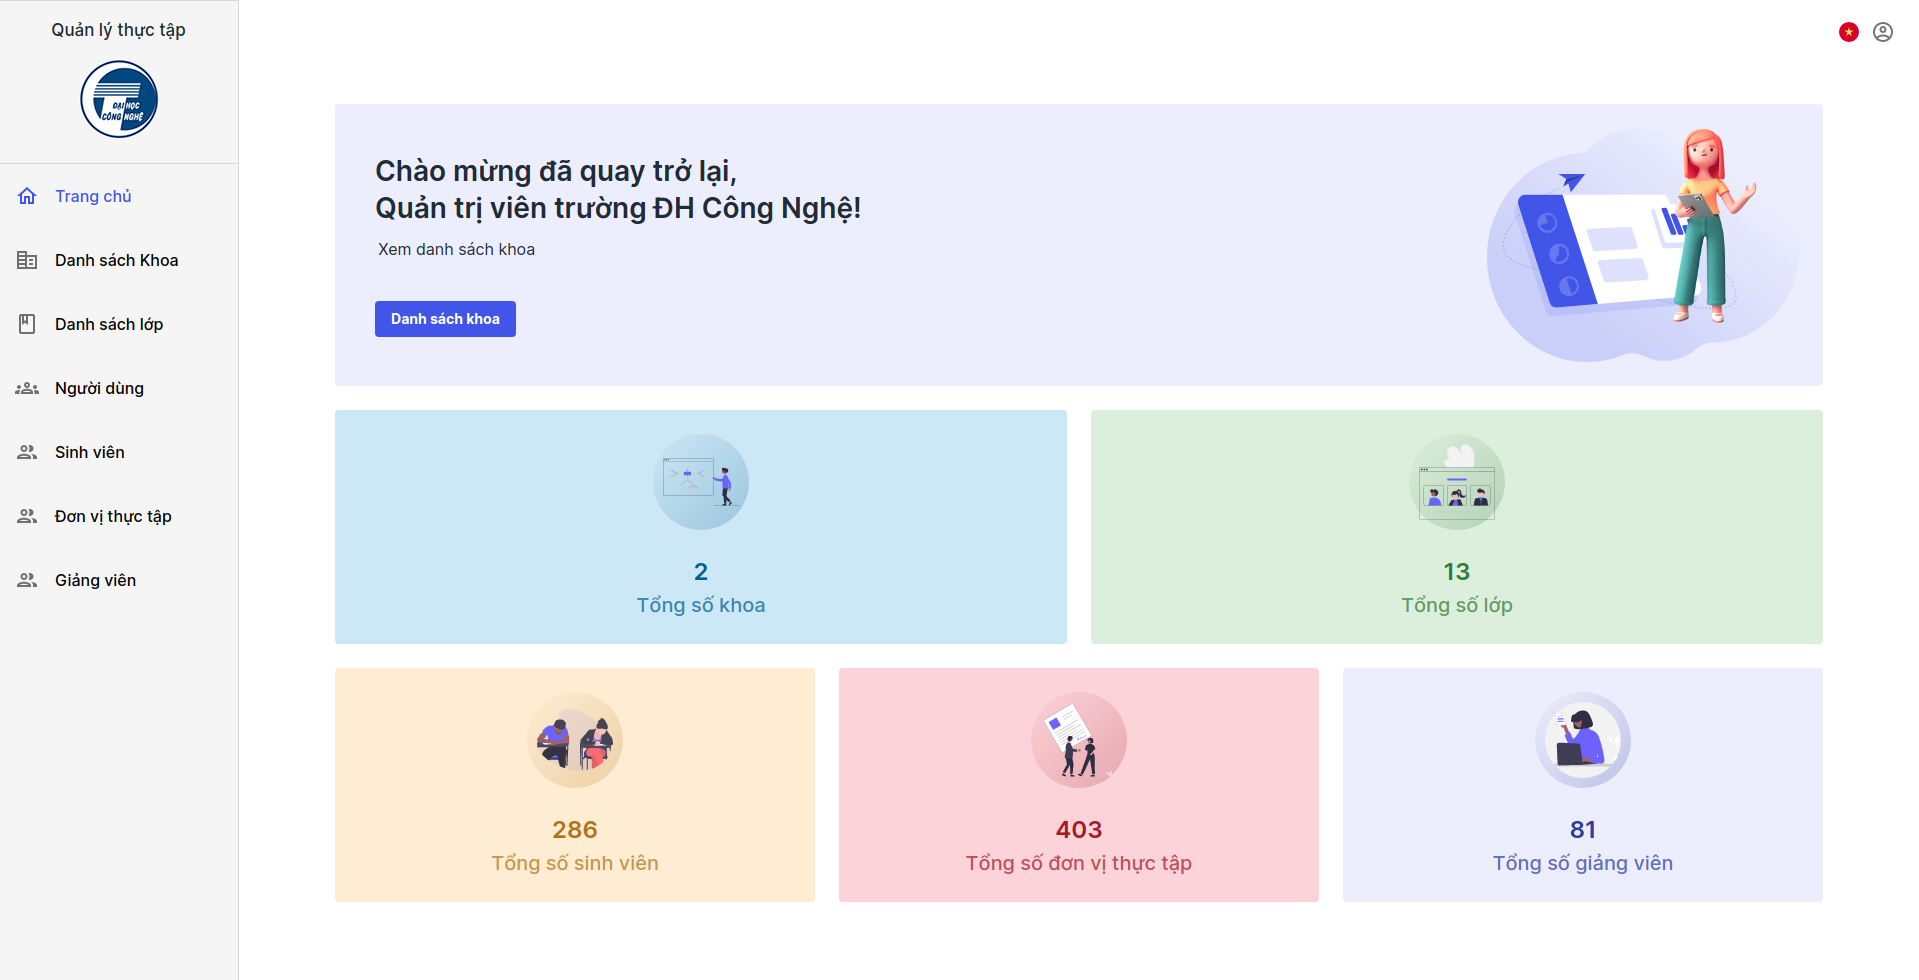
\includegraphics[width=\linewidth]{./images/image83.png}
	\caption{Màn hình dashboard của quản trị viên hệ thống}
	\label{fig:sys_dashboard}
\end{figure}

\begin{figure}[H]
	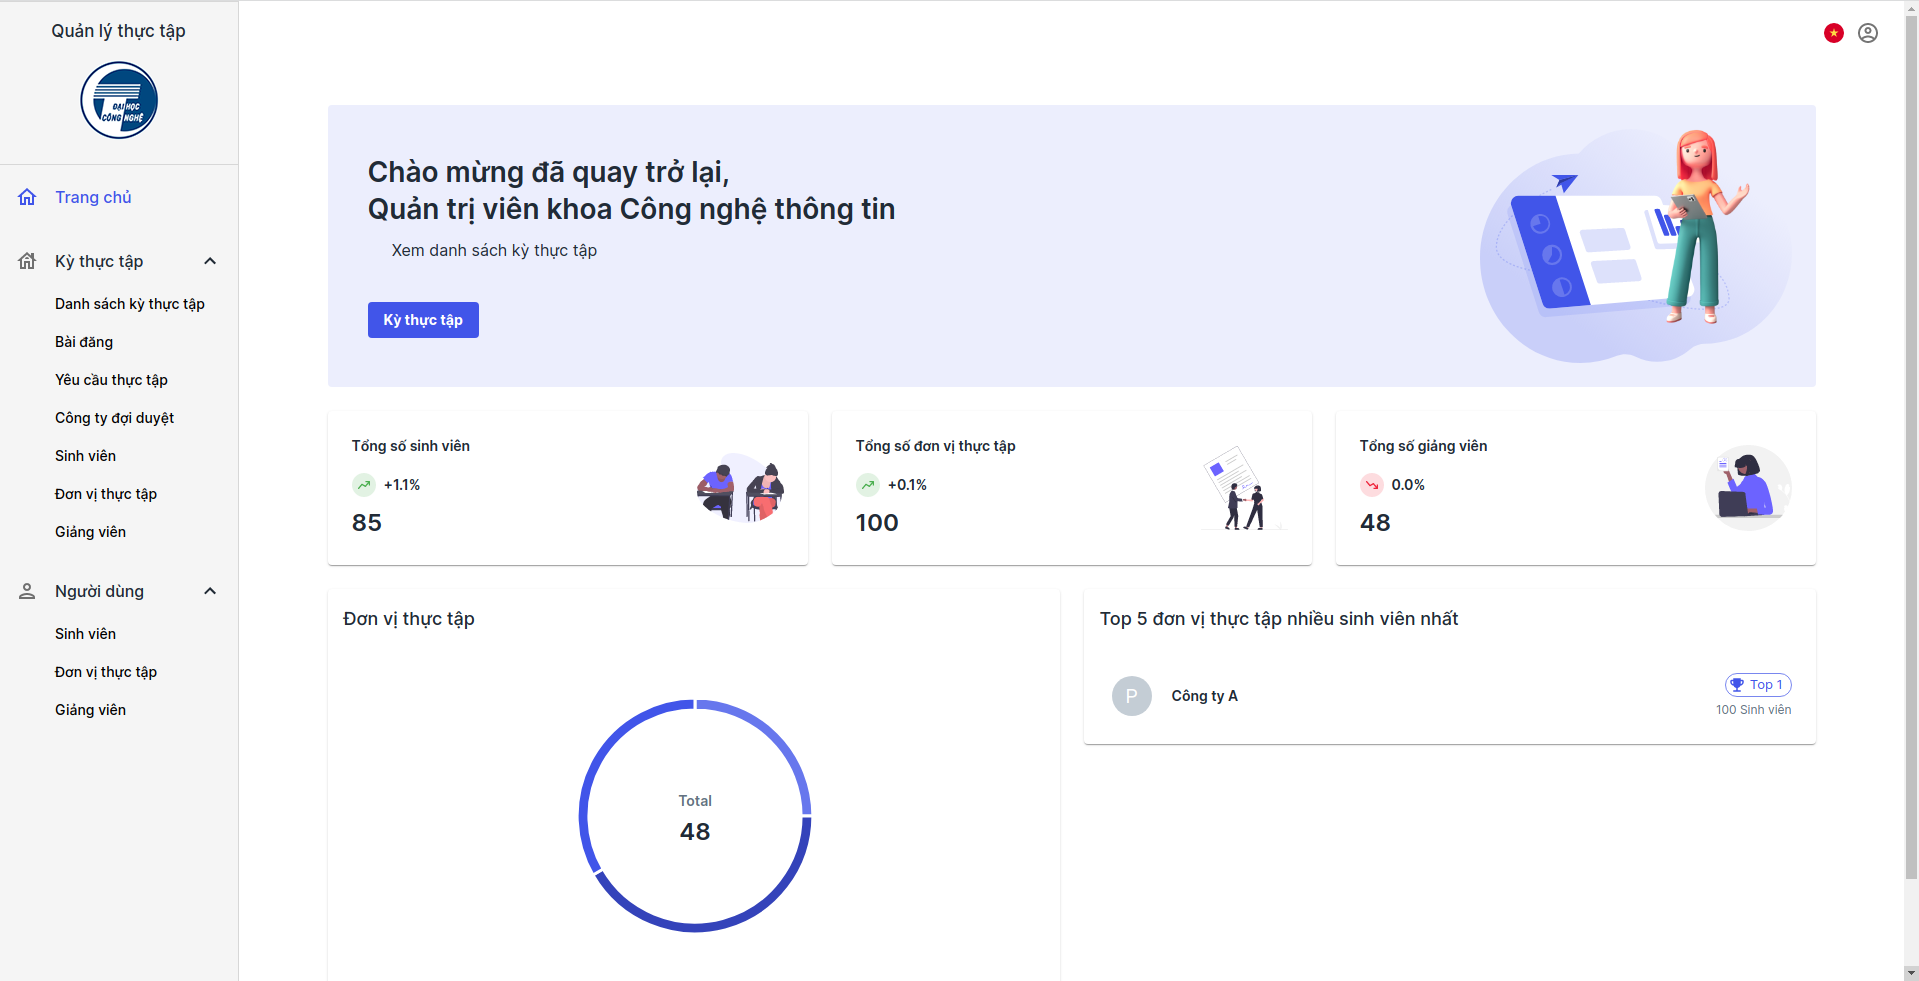
\includegraphics[width=\linewidth]{./images/image82.png}
	\caption{Màn hình dashboard của quản trị viên khoa}
	\label{fig:org_dashboard}
\end{figure}

\begin{figure}[H]
	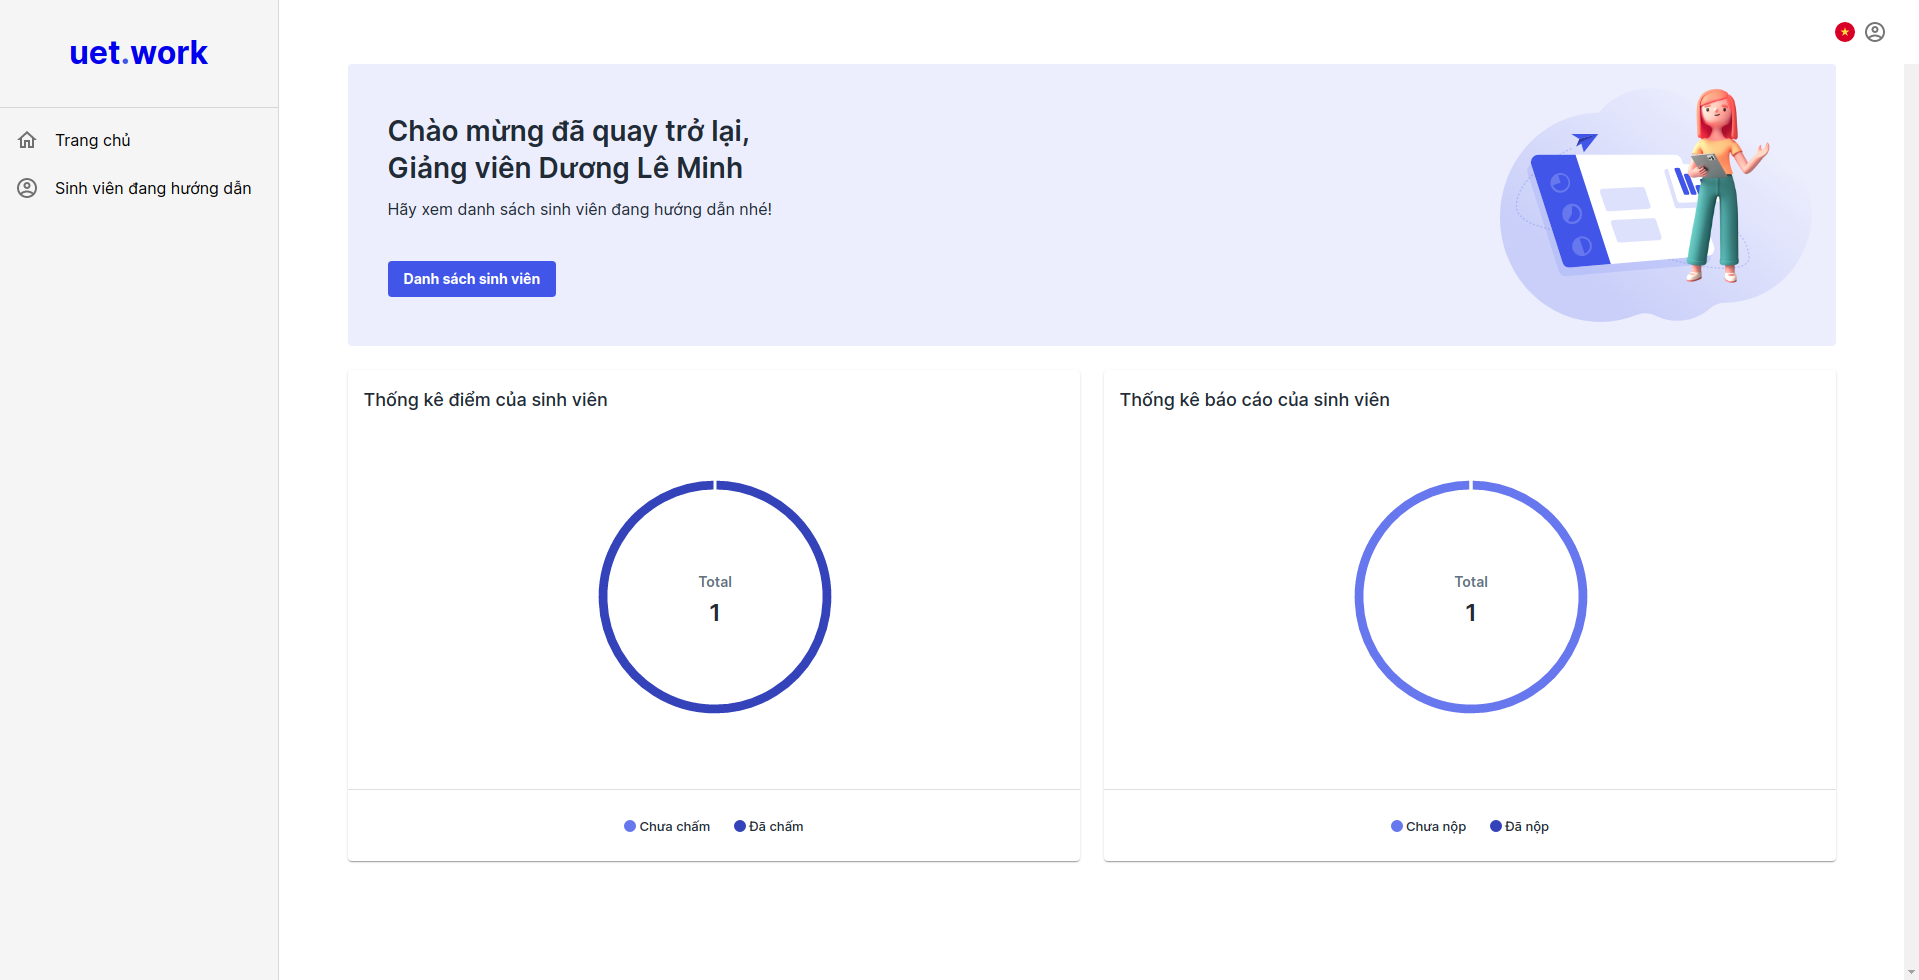
\includegraphics[width=\linewidth]{./images/image85.png}
	\caption{Màn hình dashboard của giảng viên}
	\label{fig:lecturer_dashboard}
\end{figure}

\begin{figure}[H]
	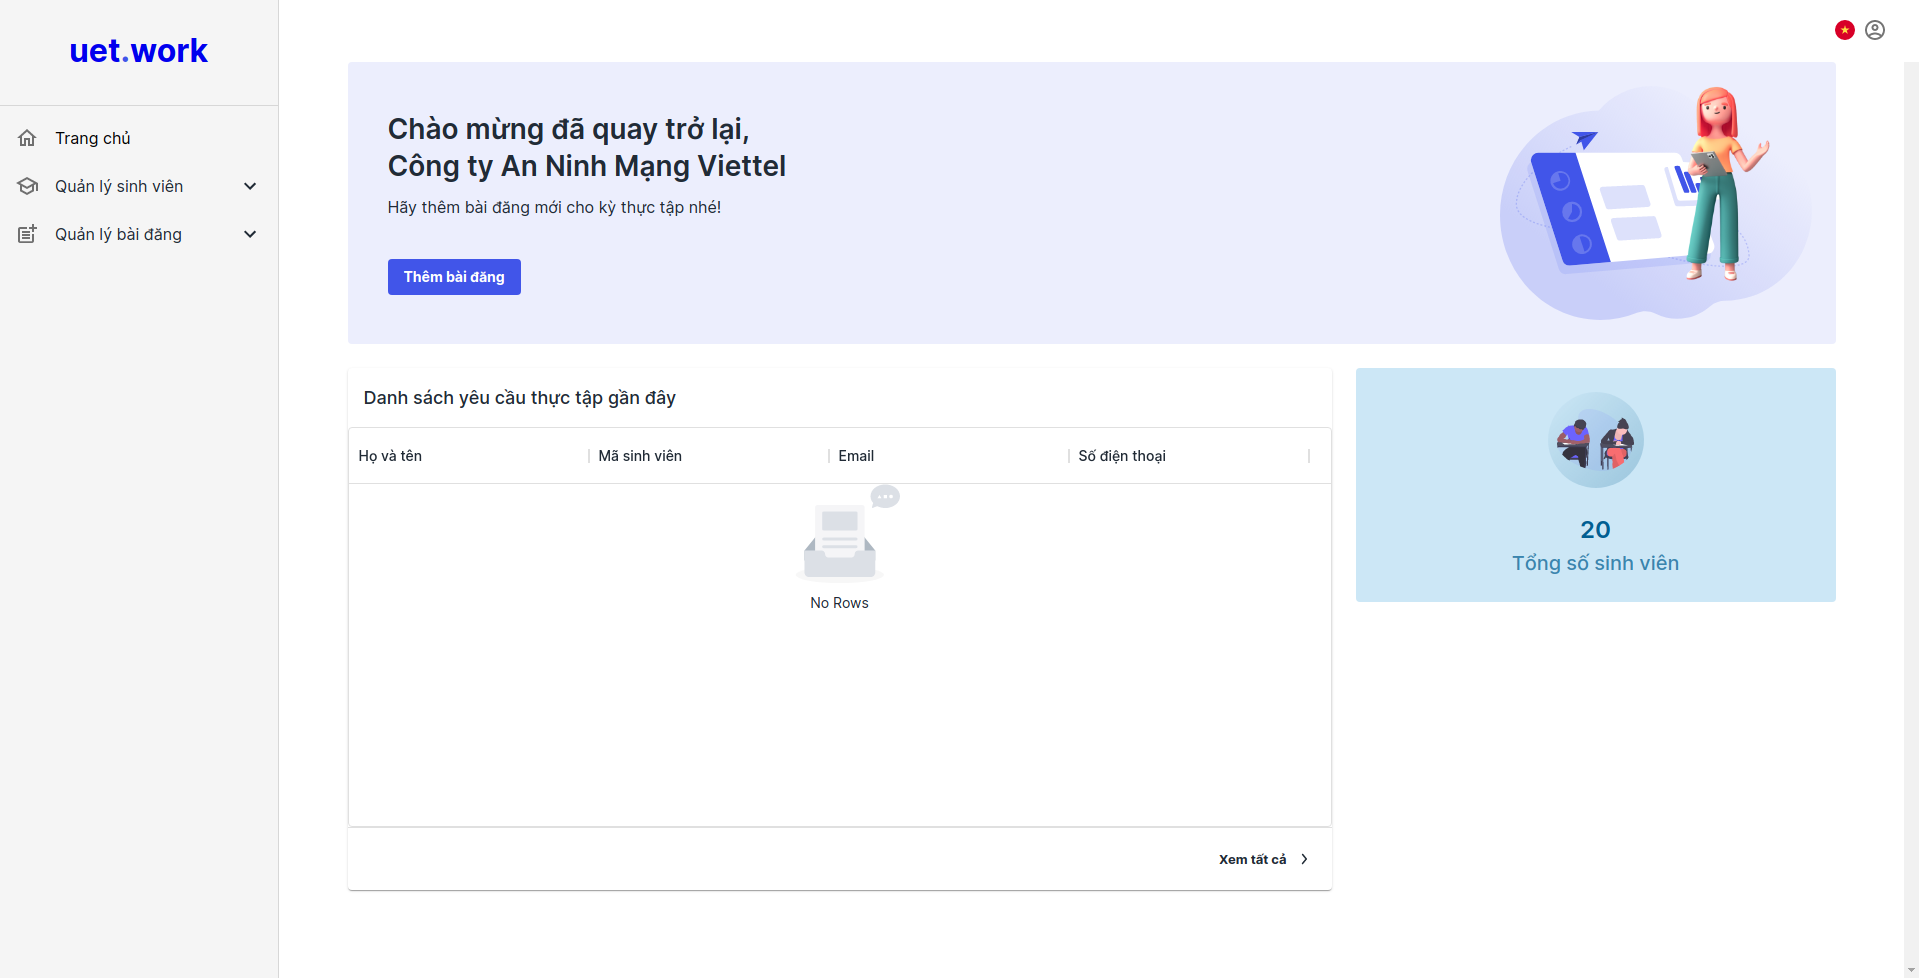
\includegraphics[width=\linewidth]{./images/image84.png}
	\caption{Màn hình dashboard của công ty}
	\label{fig:partner_dashboard}
\end{figure}



\hypertarget{ux111a-nguxf4n-ngux1eef-1}{%
	\subsection{Giao diện hỗ trợ đa ngôn ngữ}\label{ux111a-nguxf4n-ngux1eef-1}}


Hệ thống cũ chưa nhất quán về ngôn ngữ hiển thị cho giao diện, khiến người dùng có trải nghiệm chưa được tốt khi sử dụng hệ thống. Hình \ref{fig:old_admin_page} cho thấy giao diện màn hình quản trị viên, phần sidebar hiển thị hoàn toàn bằng tiếng Anh, nhưng phần nội dung lại được hiển thị bằng tiếng Việt.

\begin{figure}[]
	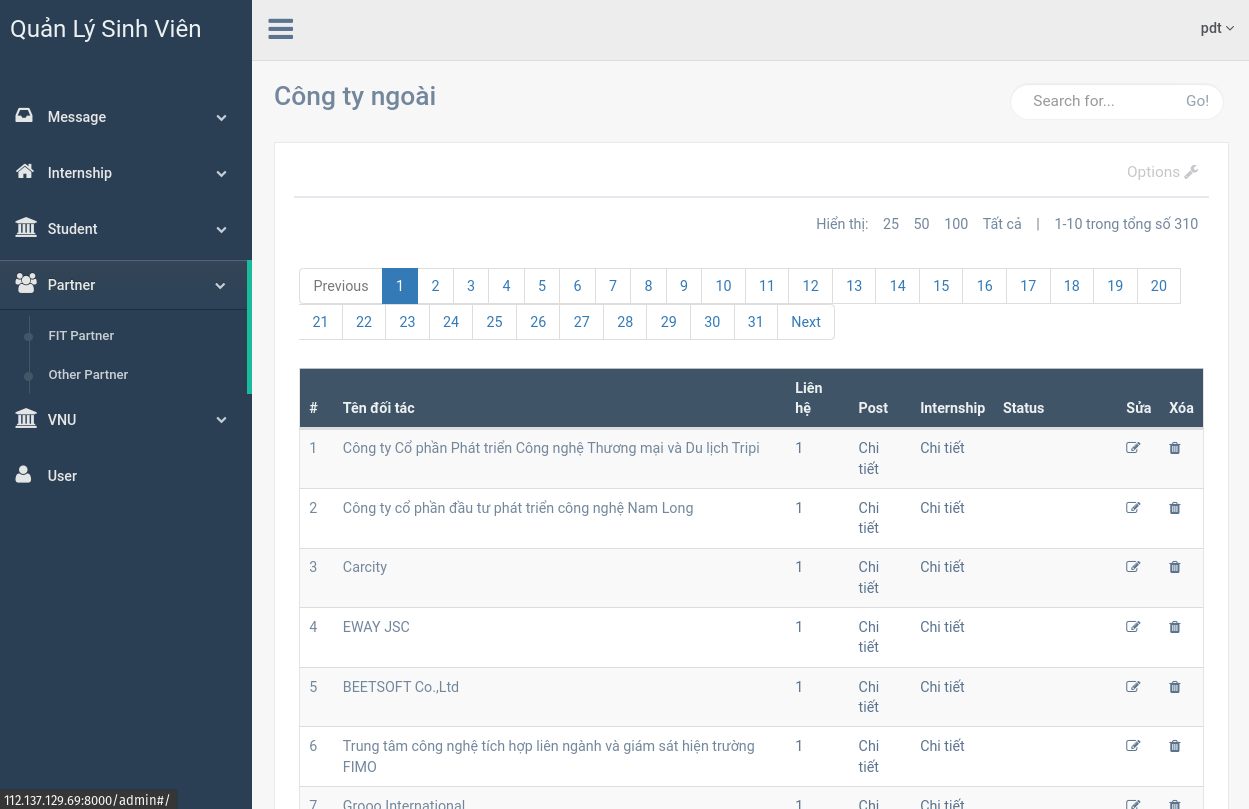
\includegraphics[width=\linewidth]{./images/old_admin_page.png}
	\caption{Màn hình quản trị viên của hệ thống cũ}
	\label{fig:old_admin_page}
\end{figure}

Hệ thống mới đã đặt mục tiêu hỗ trợ giao diện đa ngôn ngữ từ thời điểm ban đầu. Trên giao diện, người dùng có thể lựa chọn ngôn ngữ phù hợp nhất với bản
thân. Với tính năng này, sinh viên quốc tế có thể sử dụng hệ thống dễ dàng hơn.

Để làm được việc này, phần client sử dụng thư viện i18next\footnote{\url{https://www.i18next.com/}}, cho phép nhà phát triển tạo ra một file chứa toàn bộ nội dung được dịch.

Hình \ref{fig:en_page} và \ref{fig:vi_page} mô tả 2 màn hình tiếng Anh và tiếng Việt của hệ thống.

\begin{figure}[]
	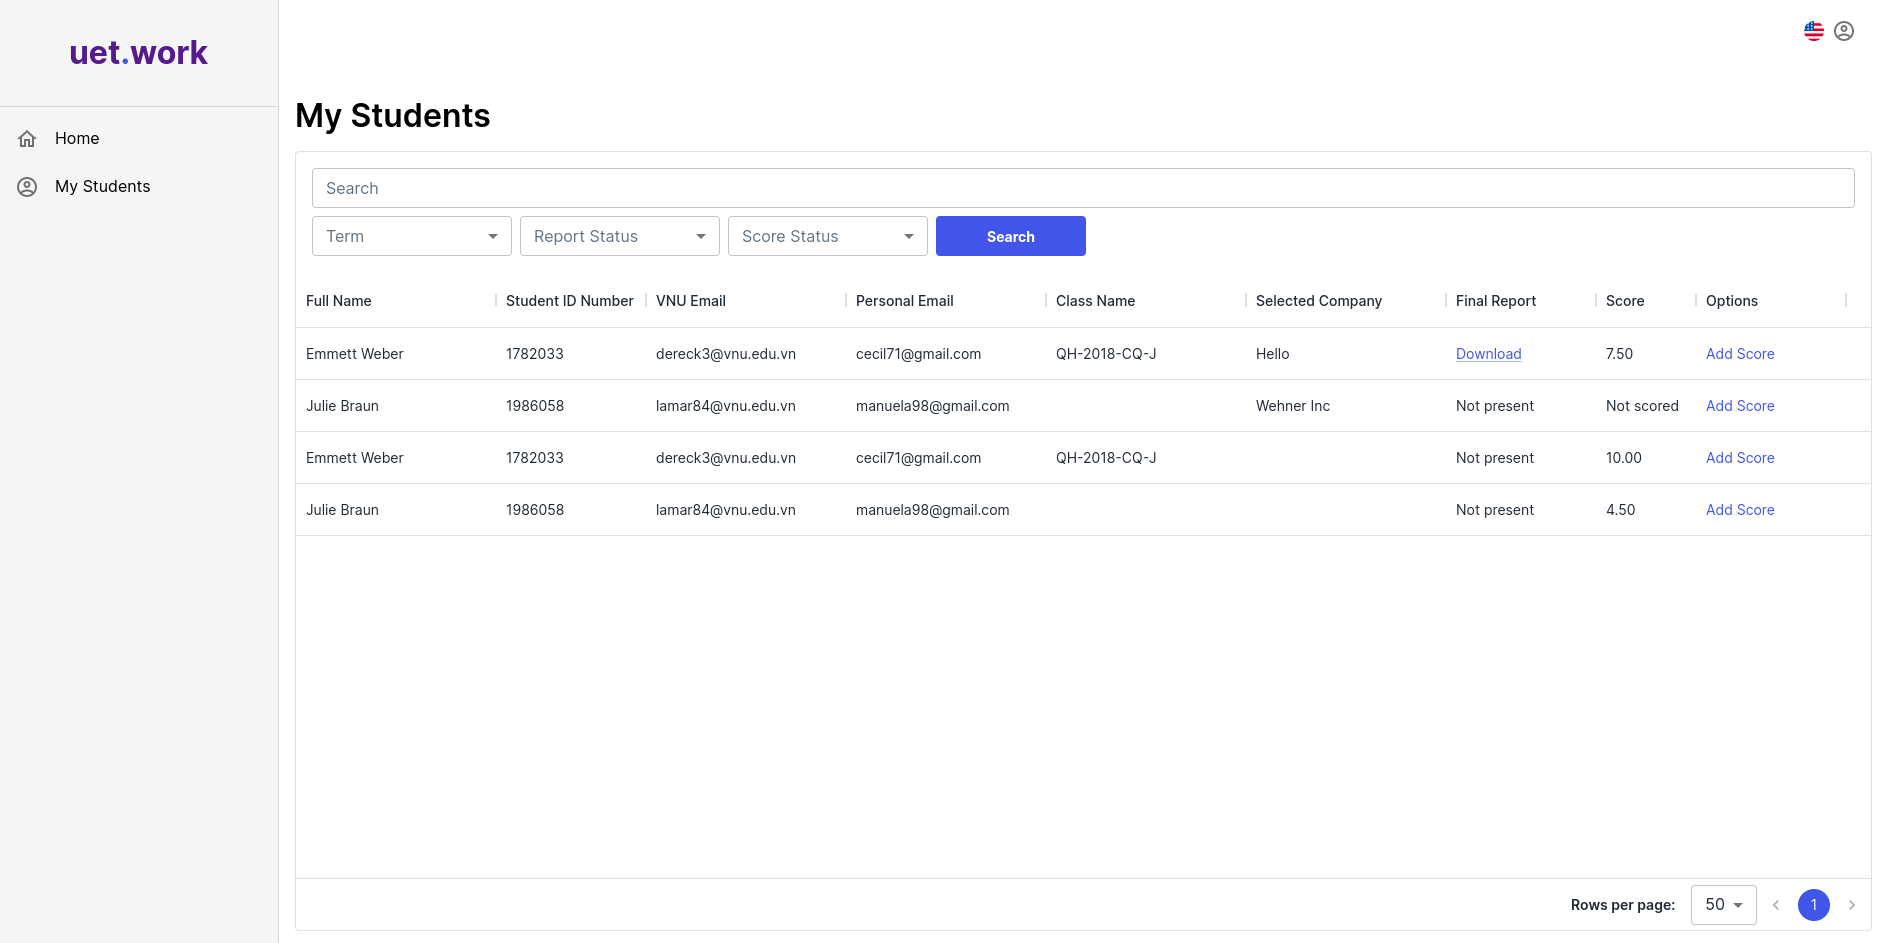
\includegraphics[width=\linewidth]{./images/image13.png}
	\caption{Màn hình hệ thống (tiếng Anh)}
	\label{fig:en_page}
\end{figure}

\begin{figure}[]
	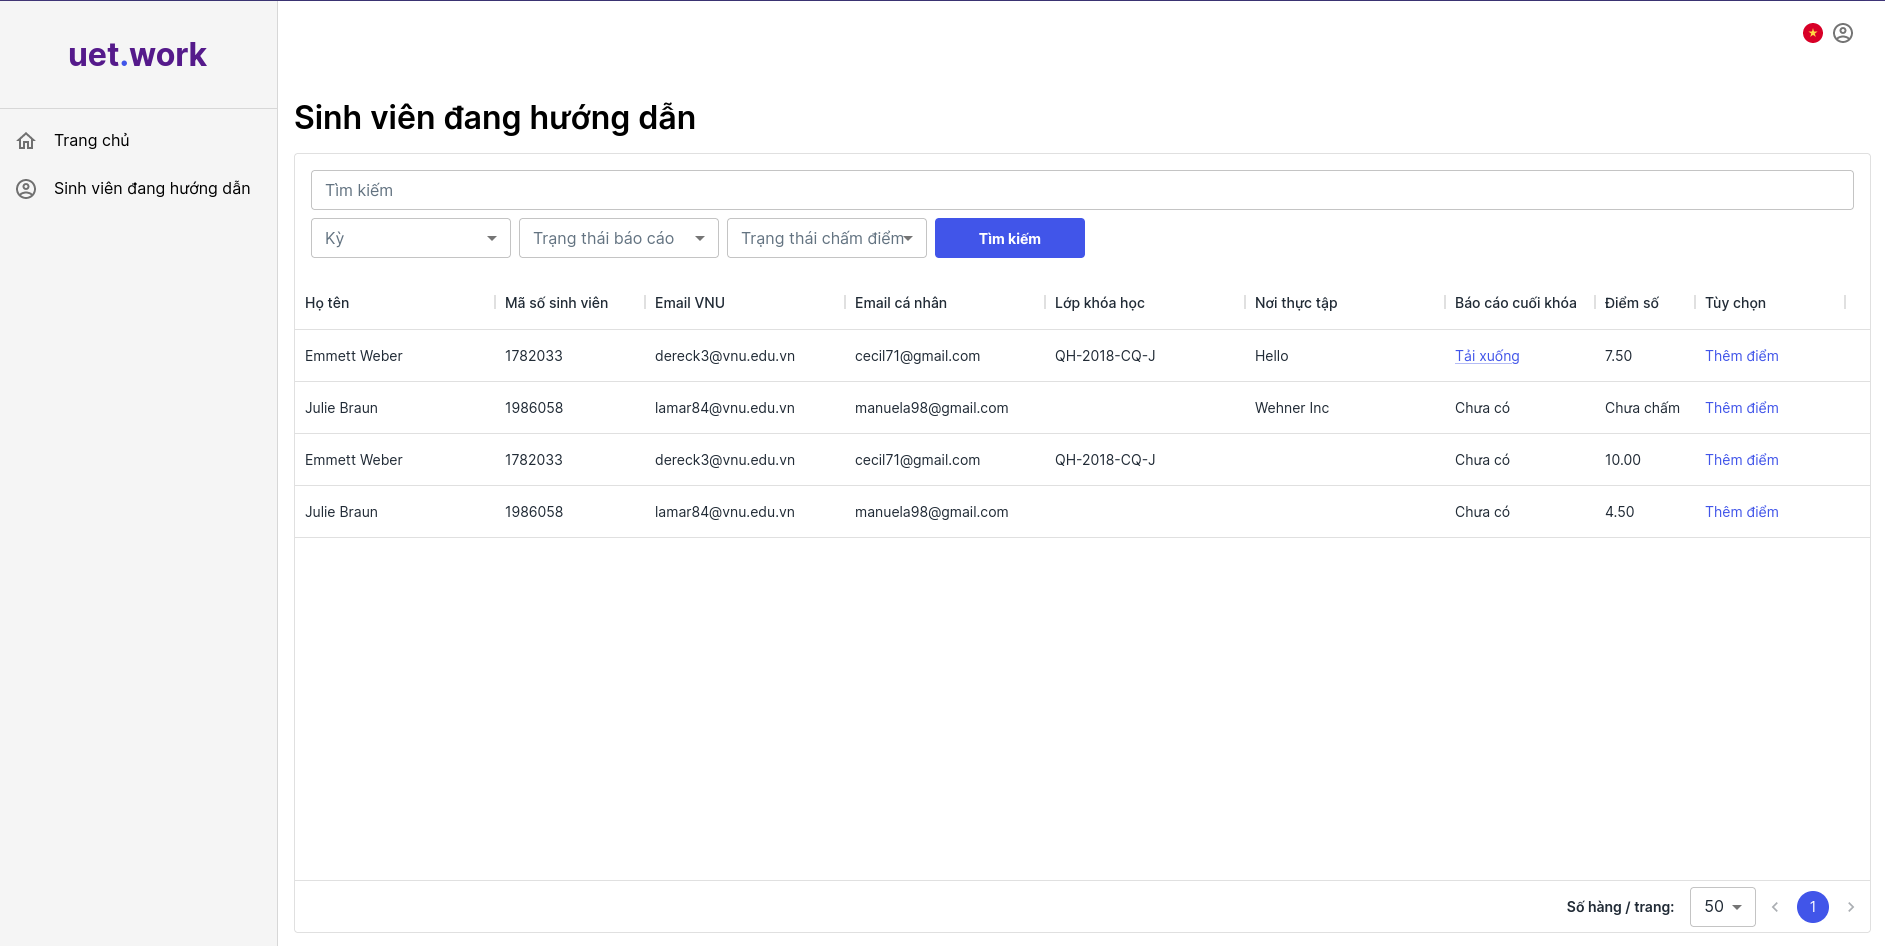
\includegraphics[width=\linewidth]{./images/image12.png}
	\caption{Màn hình hệ thống (tiếng Việt)}
	\label{fig:vi_page}
\end{figure}

\end{document}